\documentclass[12pt]{article}
\usepackage{../template/NotesTeX}
\graphicspath{ {/home/ab/school/notes/chemmat121/} }
\begin{document}

\title{Chemmat 121}
\author{Alexander Bailey}
\emailAdd{alexkingstonbailey@gmail.com}
\maketitle
\flushbottom

\section{Deformation and structure of solids}
\subsection{Strength}
How much force can a material withstand before it fails?
That's a materials strength.
A material can fail in several ways but the two most common are fracturing and permanent deformation.

  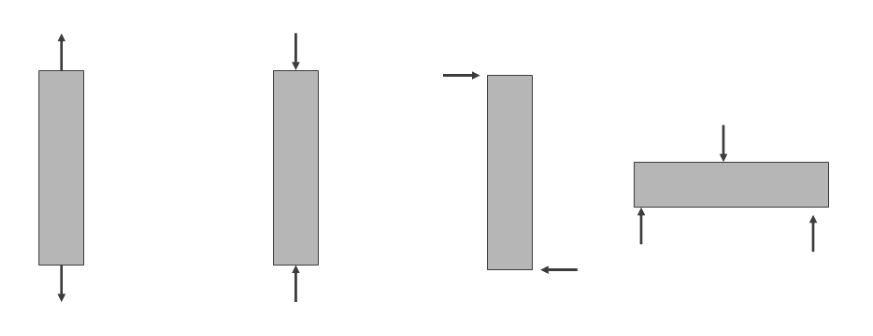
\includegraphics[scale=0.5]{force-types}
  \begin{center}
    Some types of force that a material/object can undergo

    From left: Tension, Compression, Shear and a Combination.
  \end{center}

\subsection{Stress}
Engineers typically talk about stress instead of forces because stress is just a force proportional to its area.
Stress is represented by the greek letter sigma ($\sigma$) and is given by the force (F) divided by the cross-sectional area (A).

\marginnote{Cross-sectional area is the area that is perpendicular to the applied force}

\begin{equation*}
  \sigma = \frac{F}{A} \\
\end{equation*}

\begin{example}
  \begin{flalign*}
    \text{Given: } m=25\unit{kg}, d=10\unit{mm} \\
    A = \pi r^2 \\
    A = \pi \times \frac{(0.01)^2}{2} \\
    F = 25 \times 9.81 \\
    \sigma = \frac{F}{A} \\
    \sigma = 3,120,000 \unit{Pa} \\
    \sigma = 3.12 \unit{MPa} \\
  \end{flalign*}
\end{example}

\begin{marginfigure}
  \vspace{-8cm}
  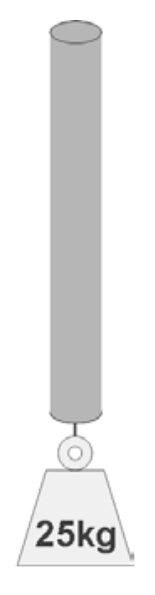
\includegraphics[scale=0.3]{stressexample}
\end{marginfigure}

\subsection{Strain}
Strain is how long something gets compared to its original size.
Stress and strain are related very closely and the stress against strain graph is a very important thing to materials engineering.
Strain is given by the change in length over the original length.

\begin{equation*}
  \epsilon = \frac{\Delta L}{L_o} 
\end{equation*}  

Strain is unitless but is commonly expressed as a percentage (\%).

\begin{example}
  \begin{align*}
    \epsilon &= \frac{\Delta L}{L_o} \\
             &= \frac{100.32\unit{mm}-100\unit{mm}}{100\unit{mm}} \\ 
            &= \frac{0.32\unit{mm}}{100\unit{mm}} \\ 
            &= 0.0032 \\
            &= 0.32\% \\ 
  \end{align*}
\end{example}

\subsection{Stress-Strain Curve}
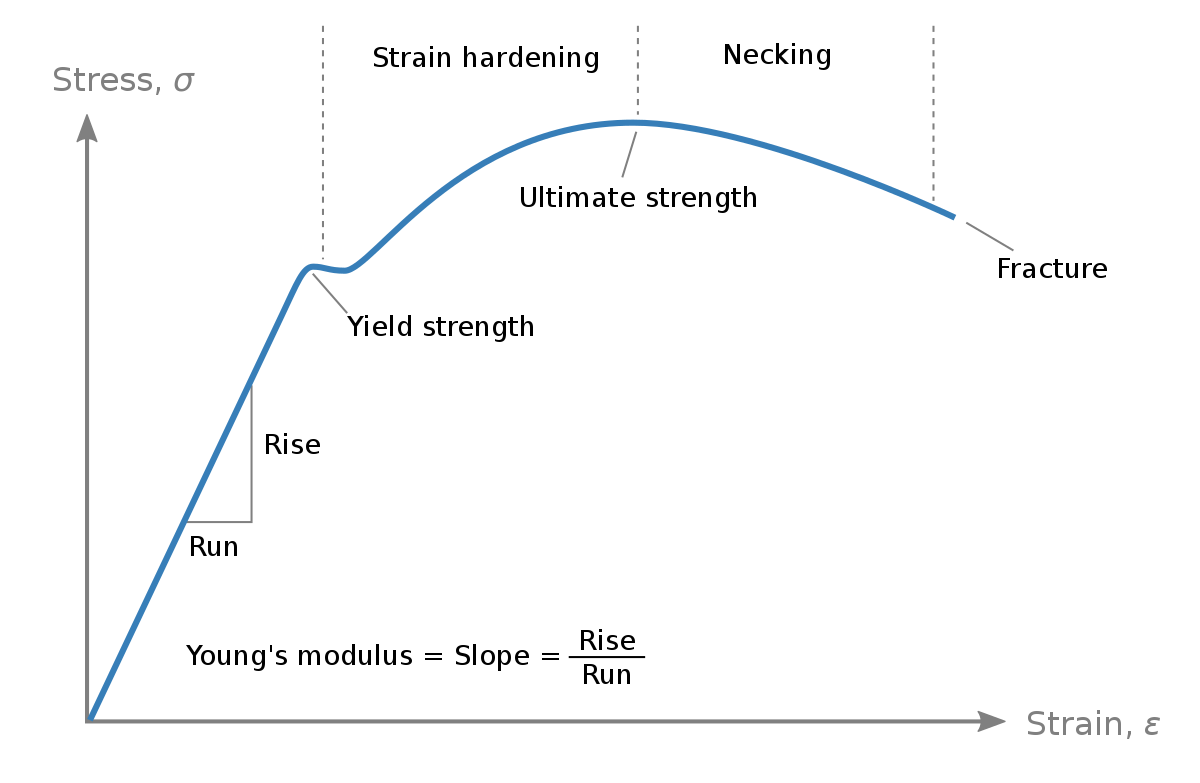
\includegraphics[scale=0.3]{stressvsstrain}

\en{The area under the curve is $F\times d$ and gives the `toughness' which is approximately the energy required.}[-8cm]

\en{Necking is a localised reduction in thickness, which reduces diameter, which reduces area, increasing stress. This causes it to fail.}[-4cm]

\subsection{Poisson's Ratio}
Poisson's ratio is the relationship between deformation for a given material. 
It is a measure of the Poisson effect, that describes the expansion or contraction of a material in directions perpendicular to the direction of loading. 
It has no units and is represented by the greek character `nu' ($\nu$).
For most materials $\nu \approx 0.3$.

\begin{equation*}
\nu = \frac{-\epsilon_x}{\epsilon_z}
\end{equation*}

\subsection{Young's Modulus}
The Young's Modulus of a material is a measure of the `stiffness'. 
It is the gradient of the elastic part of the stress-strain curve for a given material.
It has units of Pascals (Pa) and is represented by the capital letter E. 

\begin{equation*}
  E = \frac{\Delta \sigma}{\Delta \epsilon} 
\end{equation*}
\subsection{Steel}
Steel has what is called a `discontinuous yield'.  
This means at the yield strength there is a bit of `noise' and it moves a little randomly before becoming nonlinear. 

\subsection{0.2\% Proof Stress}
The 0.2\% Proof Stress of a material is a geometrical construct that is used when the yield stress of a material cannot be properly determined. 
It is a very slight overestimate (generally) that can be calculated by drawing a line parallel to the actual curve at a strain of $0.002$ and finding the intersection with the original curve.
This stress value is the approximation. 

\subsection{Safety Factor}
The safety factor is a scalar value that demonstrates how much more stress a material can hold relative to the requirement. 
I.e. if, for example, $F \approx 1000\unit{N}$ the engineers might pretend $F = 2000N$. 
This would gie a safety factor of 2.

When the conditions of the material are more uncertain, you would want a higher safety factor.

\subsection{Engineering Stress vs Real Stress}
In engineering, we draw a stress-strain graph as going `down' after the ultimate tensile strength.
In reality, because of the effect of necking, it goes up after this.
As engineers, we use the model because it is easier to handle theoretically.

\subsection{Ductility}
Ductility is a measure of how much something can deform elastically (with 100\% recovery / without permanent deformation).
The stress-strain graph of a ductile material will have a longer elastic section while a more brittle material (less ductile) will have a shorter one.
It is generally described by one of two equations: 

\begin{center}
  \textbf{Percentage Elongation}
\end{center}
\begin{equation*}
  = \frac{\Delta L}{L_o} \times 100\% 
\end{equation*}

\begin{center}
  \textbf{Percentage Reduction in Area}
\end{center}
\begin{equation*}
  = \frac{\Delta A}{A_o} \times 100\% 
\end{equation*}

\section{Microstructure and mechanical properties}
\subsection{Crystal Structure}
\begin{definition*}
  If a material is crystalline, the atoms of a material have \textbf{LONG RANGE ORDER}. 
  This means the material is made up of a crystal lattice made of repeating units called `unit cells'. 
\end{definition*}

There are 14 possible crystal arrangements but this course will only look at three. 
We describe arrangements by looking at the unit cell. 
The unit cell is a tessellating shape that has all the information to describe the entire lattice.

The unit cell has 4 important properties: 
\begin{itemize}
  \item Number of atoms 
  \item Co-ordination Number (The number of neighbours for the unit cell)
  \item Unit Cell Dimension (The length of each side of the cell written `a')
  \item Atomic Packing Factor (Amount of space taken up by the atoms)
\end{itemize}

\begin{equation*}
  a = \text{ Atomic Packing Factor } = \frac{\text{volume of atoms}}{\text{volume of unit cell}}
\end{equation*}

\subsubsection{Body Centered Cubic} 
Body Centered Cubic (BCC) has one atom at each corner of a cube and one right in the middle.
\begin{marginfigure}
  \vspace{ -1cm }
  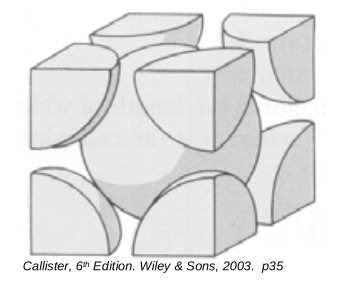
\includegraphics[scale=0.15]{bcc}
\end{marginfigure}

\begin{itemize}
  \item Number of Atoms = $2 = 1 + 8 \times \frac{1}{8}$
  \item Co-ordination Number = 8 
  \item Unit cell dimension = $\frac{4R}{\sqrt{3}}$
  \item APF = 0.68 = 0.68\%
\end{itemize}

\subsubsection{Face Centered Cubic}
Face Centered Cubic (FCC) has one atom at each corner of a cube and one in the middle of each face of the cube.
\begin{marginfigure}
  \vspace{ -1cm }
  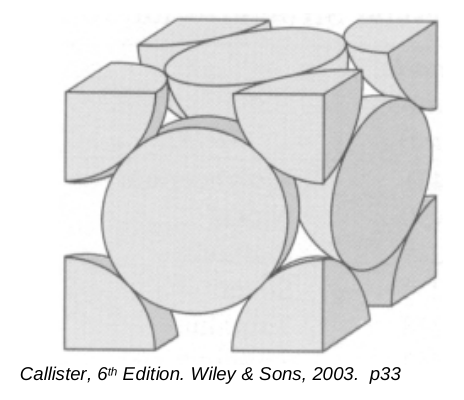
\includegraphics[scale=0.11]{fcc}
\end{marginfigure}

\begin{itemize}
  \item Number of Atoms = $4$
  \item Co-ordination Number = 12 
  \item unit cell dimension = $\frac{4R}{\sqrt{2}}$
  \item APF = 0.74 = 0.74\%
\end{itemize}

\subsubsection{Hexagonal Close Packed}
Hexagonal Close Packed (HCP) is a prism shape with hexagonal arrangements of atoms layered up.
\begin{marginfigure}
  \vspace{ -1cm }
  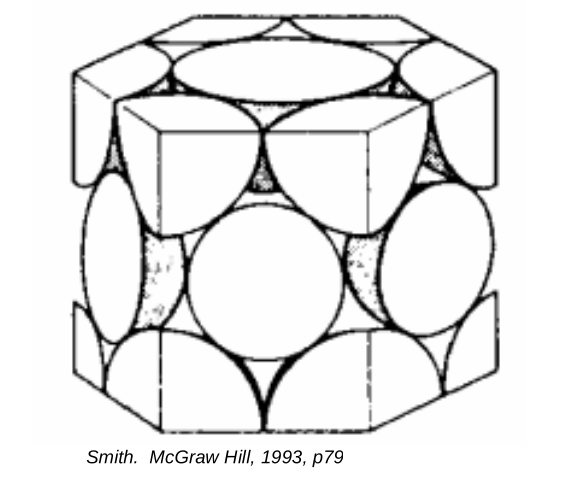
\includegraphics[scale=0.1]{hcp}
\end{marginfigure}

\begin{itemize}
  \item Number of Atoms = $6$
  \item Co-ordination Number = 12 
  \item APF = 0.74 = 0.74\%
\end{itemize}

\subsection{Density}
Density is the degree of compactness of a substance. 
The amount of mass you get for a given volume.
The density of a material is its mass divided by its volume.
\begin{equation*}
  \rho = \frac{n.A}{V_c.N_a}
\end{equation*}
Where $n$ is the number of atoms per unit cell, $A$ is the atomic mass of the material, $V_c$ is the volume of the unit cell ($a^3$) and $N_a$ is Avrogado's Number.

\begin{example}
  Iron
  \begin{gather*}
    a = 0.286\unit{nm }, n = 2 \\
    \rho = \frac{ 2 \times 55.85 }{(2.86\times10^{-8})^3 \times 6.023 \times 10^{23}} \\
    \rho = 7.92\unit{g.cm}^{-3}
  \end{gather*}
  The real density of iron is 7.87$\unit{g.cm}^{-3}$ so this is a good estimate.
\end{example}

\subsection{Polymorphism}
Materials that can exist in more than one crystal form (can have lattices made up of different unit cells) are called polymorphic. 
For example, Iron at room temperature has a BCC structure but at $912^\circ$C it has an FCC structure.

\newpage
\subsection{Planes, Directions and Positions}
Navigation around our crystal structures is based on a typical x,y,z orthogonal axis. 
We can denote the postition of an atom using a typical three dimensional vector. 
By convention, positions are denoted with round brackets.

\begin{marginfigure}
  \vspace{-1.5cm}
  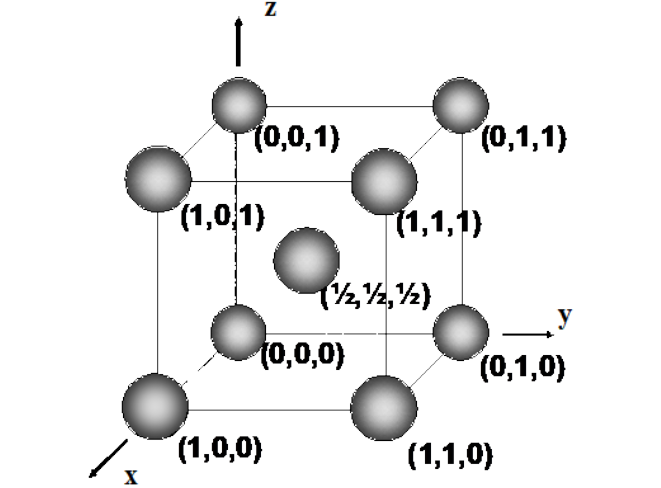
\includegraphics[scale=0.2]{positions}
\end{marginfigure}


\subsubsection{Directions}
Directions in the lattice are defined with square brackets $[u,v,w]$.

\begin{enumerate}
  \item Draw a vector from the origin for the direction 
  \item Project the length of the vector onto the unit cell axes 
  \item Put this in terms of the coefficients 
  \item Convert to integers (multiply by a constant)
  \item Put in square brackets 
\end{enumerate}

\begin{example}
  Projecting the length of the vector onto axes:
  $1a$ $0b$ $\half c$

  Put this in terms of co-efficients:
  $1$ $0$ $\half$

  Convert to integers (multiply by two):
  2 0 1

  Put in square brackets:
  $[201]$
\end{example}

Note: Negative directions will have a bar over them (read `bar').  

\begin{equation*}
[1\bar{1}0]
\end{equation*}

\subsubsection{Planes}
Planes in the lattice are defined by \textbf{Miller Indices} $(h,k,l)$.

\begin{enumerate}
  \item Work out the intercepts of the plane on the unit cell 
  \item Take reciprocals of the intercepts 
  \item Convert to integers (multiply by a constant)
  \item Put in round brackets 
\end{enumerate}

\begin{example}
  Intercepts: $1$ $-1$ $\infty$

  Reciprocals: $1$ $-1$ $0$

  Integers: $1$ $-1$ $0$

  Round Brackets: $(1\bar{1}0)$
\end{example}

\subsubsection{Families}
You can denote the `family' of a plane (all of the planes made up with these values). 
Families of planes are denoted with curly brackets e.g. Cube Faces $\{100\}$.
Families of directions are denoted with angle brackets e.g. $<100>$.

\subsection{Slip, Theoretical Strength and Defects}
Recall that there are two types of deformation: Elastic and Plastic (In-elastic).
Elastic Deformation springs back (recovers), Plastic Deformation does not.

At the atomic level, Elastic Deformation is merely stretching the atomic bonds.
Any further deformation is permanent (plastic, past the yield point) and results from a process called \textbf{slip}.
In plastic deformation, atomic bonds are broken (and remade).

\subsubsection{Theoretical Strength}
We can can calculate the \textit{theoretical} strength of a material by evaluating the amount of energy needed to break and remake the atomic bonds.
This is not a very good approximation. For example, the theoretical shear strength of pure iron is 10,000MPa but the measured shear strength of pure iron is 20MPa...
Why is this? Imperfections.

\subsection{Imperfections}
There are a number of a different imperfections that DO happen within a lattice containing millions of atoms.
This is what causes our theoretical strength and theoretical density to be off. 
It is EXTREMELY difficult to get `pure' anything so this is true for any sample.

\begin{itemize}
  \item Point Defects
    \begin{itemize}
      \item Vacancy
      \item Substitution
      \item Interstitial Atom
    \end{itemize}
  \item Planar Defects (Dislocations, $\bot$)
    \begin{itemize}
      \item Edge Dislocation
      \item Screw Dislocation
    \end{itemize}
\end{itemize}

A vacancy is simply a missing atom in the lattice.
A substitution is when a different atom is in the place of the atom that should be there. 
Interstitial atoms are atoms that occupy a normally unoccupied site in a crystal lattice.

\subsection{Slip}
\begin{center}
  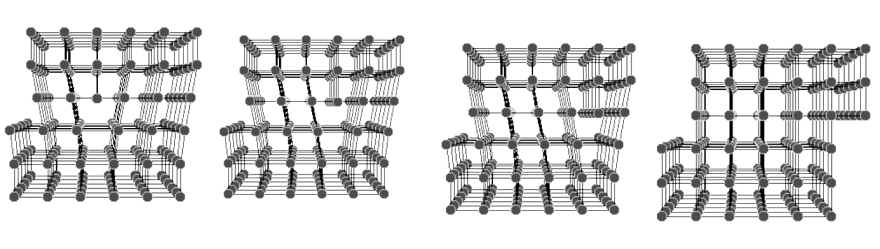
\includegraphics[scale=0.2]{slip}
\end{center}

\marginnote{Explaining how Slip works is a common exam question. Draw these!}[-1.7cm]

The model of slip we will use is the movement of dislocations.
The movement of dislocations means that slip can occur more easily than in a perfect arrangement of atoms.
Easy slip means that a material is easily plastic deformed, this means it is \textit{ductile}.


\subsubsection{Slip Systems}
Slip (dislocation movement) occurs most easily on closepack planes and in closepacked directions.
Not all systems have closepacked planes so slip happens on the \textit{closest} packed plane  

A slip system is a combination of planes and directions.
For FCC, the closepacked planes are $\{111\}$\mn{A family of planes}.
The closepacked directions on these planes are $<110>$\mn{A family of directions}.

Hence, the main slip system for FCC is: $\{111\}<110>$

The main slip system for BCC is: $\{110\}<111>$

HCP structures have closepacked planes but they are all parallel.
Slip is very difficult so HCP metals are often brittle. 

\subsection{Microstructure}
Engineering components are very rarely single crystals, this means they are polycrystalline (many crystals).
Most metals have at some point been molten and as they solidify they form many crystals.

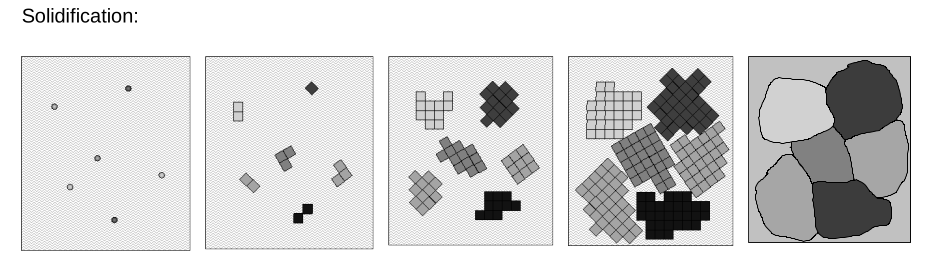
\includegraphics[scale=0.4]{solidification}

The name for the individual pieces is nucleus.
If they have lost enough energy (cooling down) they might form nuclei when they bump together.
This happens in the 2nd panel, you can call them "Baby Crystals".

The separate sections are `perfect crystals' (but they still contain defects) and in the 4th panel they are \textbf{equiaxed}. 
This means they are roughly equal in each axis and of the same size (roughly spherical/of the same size).
Each one of these crystals is called a `grain'.  
We can then talk about \textbf{Grain Structures} within a metal and \textbf{Grain Boundaries}.

When one grain meets another, the atoms are not perfectly aligned. 
This means there is a little extra energy due to the atomic bonds being incomplete or out-of-equilibrium.
This makes the grain boundary a `high energy region'.

\subsubsection{Nucleation}
When the grains form from a molten state it is called \textbf{nucleation}. 
This can occur on another solid material or in solution. 
It is quite rare to occur in solution on its own but it is called \textbf{Homogeneous Nucleation}.
When it forms on a surface e.g. the side of a mould it is called \textbf{Heterogeneous Nucleation}.

\subsection{Casting}
\subsubsection{Sand Casting}
Sand Casting is an ancient method of casting. 
You use something (foam etc) to make a hole in the sand and then fill your `runner' (input) with molten metal until it burns away all the filler.
This will then set in the sand you can take off the `cope' or `drag' (bottom or top) and access your new sword or cannon or frypan!

\begin{center}
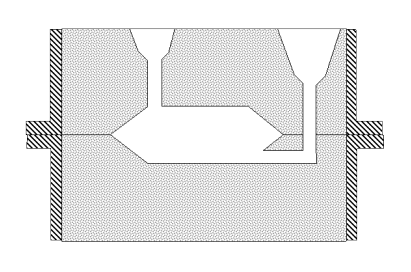
\includegraphics[scale=0.8]{sandcasting}
\end{center}
\subsubsection{Die Casting}
Die casting is a much more expensive modern method of casting.
In die casting, a permanent mould is created using machining tools out of another metal.
These moulds can be hundreds of thousands of dollars.
All forms of casting are prone to porosity however, weakening the part.

\subsection{Grain Structure Development}
Grains will mostly nucleate on the sides (walls) of the mould.
The first grains you will get are equiaxed grains.
Columnar grains will form in `columns' and stretch across the mould, possible touching the grains on the other side.
Sometimes columnar grains will form branches, these are called dendrite formations.
\marginnote{Frost will also form dendrites when it goes from gas to solid.}[-1cm]

\subsection{Metallography} 
Metallography is the study of the structure of metals. 
We use a reflective-light microscope (instead of a transmission microscope) because the metal is far too opaque to use a transmission scope.
Before we can use a microscope however you must prepare the surface.
This is to make the rough, cut surface smooth and reflective.

To allow us to see the grain boundaries, we `etch' the metal with an acid or alkali that selectively `attacks' the boundaries.
This means the boundaries will scatter light instead of reflecting it so they appear dark under the microscope. 
\marginnote{Some of the grains appear darker because they are also attacked by etching}
The general preparation process is

\begin{enumerate}
  \item Grinding
  \item Polishing (using finer and finer abrasives)
  \item Etching
  \item Cleaning (with hair-dryer, water, etc)
\end{enumerate}

\subsection{Grain Boundaries and dislocation movement}
More grains strengthen the metal because the grain boundaries stop dislocation movement (slip).
There is hence a relationship between the grain diameter and yield stress. 
This relationship is described by the \textit{Hall-Petch Equation}.

\begin{equation*}
  \sigma_y = \sigma_o + kd^{-\half}
\end{equation*}

From high school maths, you can see that this equation is linear (of the form $y=mx+c$).
On the graph $d^{-\half}$ is (typically) on the x-axis so grain size is decreasing as you move right.

\subsection{Grain deformation}
Plastically deforming grains results in work hardening.
People do this using rollers and it is called `rolling'. 
Rolling gives a rolling texture (grains are stretched out/thinner).

\begin{center}
\begin{figure}[h]
  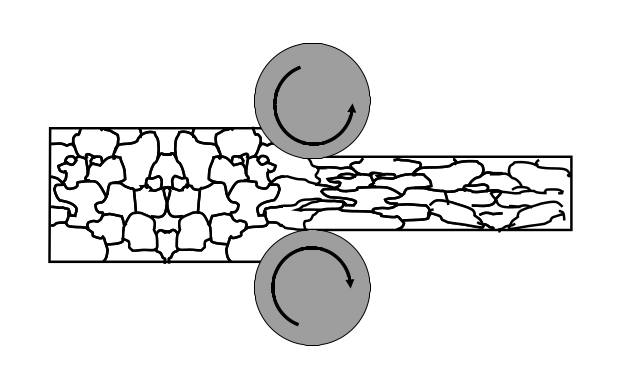
\includegraphics[scale=0.5]{rolling}

  \caption{Rolling (note the thinner grains)}
\end{figure}
\end{center}

\subsection{Work Hardening} 
As seen previously, work hardening occurs when a material is plastically deformed and released before it inevitably fractures.
Plastic deformation introduce many new dislocations.
Dislocations stop dislocations moving (and create new dislocations when moving).
The more dislocations there are, the harder it will be for them to move. 
This is, very scientifically, called a `traffic jam' and is what causes the strengthening due to work hardening.

\vspace{1cm}
Cold work is a name for the process of work hardening without heat i.e. rolling.
This causes a reduction in area as the material is because it is lengthening. 
Percentage cold work is hence the change in area over the original area. 

\begin{equation*}
  \frac{\Delta A}{A} \times 100
\end{equation*}

\subsection{Hardness}
Hardness is a resistance to a localised deformation. 
Hardness can be measured in many different ways, one popular one is the Rockwell Hardness Scales.
Geologists use Moh's which is basically "rate my rock 1-10" where 10 is diamond and 1 is Talc.

\begin{multicols}{2}
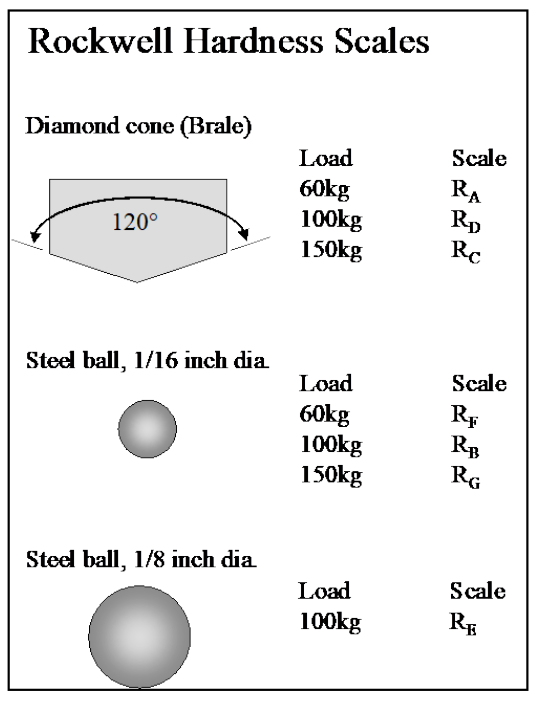
\includegraphics[scale=0.2]{rockwell}

The scales go from $R_a$ to $R_e$, where the different scales measure different levels of hardness.
Hardness has no units but you must state the scale you used i.e. 60$R_c$

You can test hardness with an indenter.
Where you make a plastic deformation with a known force behind it.

\end{multicols}

\subsection{Electrical Properties of Metals}
Electrical properties depend on atomic and crystal structures just as much as mechanical ones.
Resistivity depends on resistance (R), area (A) and length (L).
Resistance changes with temperature and so there is a second equation that has $\rho_0$ (the resistivity at room temperature), $\alpha$ (thermal co-efficient, given for each material) and $T$ (temperature).

\begin{equation*}
  \rho = \frac{RA}{L}
\end{equation*}

\begin{equation*}
  \rho_{\text{temp}} = \rho_0 (1+\alpha T)
\end{equation*}

\section{Phase diagrams and Alloying}
\section{Strengthening mechanisms}
\section{Engineering ceramics and glasses}
\section{Polymers}
\section{Failure of materials}
\section{Corrosion of metals}
\section{Engineering composites}
\end{document}
